\documentclass[12pt,a4paper,oneside]{report}

\usepackage{iftex}
\let\Bbbk\relax

\usepackage[table]{xcolor}
\usepackage{graphicx}
\usepackage{tikz}
\usepackage{geometry}
\usepackage{setspace}
\usepackage{fancyhdr}
\usepackage{titlesec}
\usepackage{tocloft}
\usepackage[hidelinks]{hyperref}
\usepackage{bookmark}
\usepackage{microtype}
\usepackage{booktabs}
\usepackage{tabularx}
\usepackage{array}
\usepackage{float}
\usepackage{longtable,colortbl,calc}
\usepackage{caption}
\usepackage{enumitem}
\usepackage{filecontents}

% Bibliographie
\begin{filecontents}{ref.bib}
@article{pandey2019machine,
  title={Machine learning applications for information systems on population studies},
  author={Pandey, A. and Others},
  journal={Journal of Data and Demography},
  year={2019},
  volume={12},
  pages={45--62}
}

@manual{hcp2024,
  title={Rapport du Recensement Général de la Population et de l'Habitat 2024},
  author={Haut-Commissariat au Plan},
  year={2024},
  organization={Haut-Commissariat au Plan}
}

@book{khoury2021data,
  title={Data Visualization and Business Intelligence with Python},
  author={Khoury, S.},
  year={2021},
  publisher={TechPress}
}

@misc{streamlit2024,
  title={Streamlit Documentation},
  author={{Streamlit Community}},
  year={2024},
  note={\url{https://streamlit.io}}
}
\end{filecontents}

\usepackage[backend=biber,style=ieee,sorting=none]{biblatex}
\addbibresource{ref.bib}

% Nomenclature / Abréviations
\usepackage[intoc,french]{nomencl}
\makenomenclature
\renewcommand{\nomname}{Liste des abréviations}

\ifPDFTeX
  \usepackage[T1]{fontenc}
  \usepackage[utf8]{inputenc}
  \usepackage{textcomp}
  \usepackage{newtxtext,newtxmath}
\else
  \usepackage{fontspec}
  \defaultfontfeatures{Ligatures=TeX,Scale=MatchLowercase}
\fi

\usepackage[french]{babel}

\geometry{
  a4paper,
  top=2.8cm,
  bottom=2.8cm,
  left=2.8cm,
  right=2.7cm,
  headheight=23pt,
  headsep=0.8cm,
  footskip=1.2cm
}

\definecolor{IbnZohrBlue}{RGB}{0,74,153}
\definecolor{HCPGreen}{RGB}{0,128,96}
\definecolor{ReportGold}{RGB}{190,140,25}
\definecolor{ReportRule}{RGB}{205,210,218}
\definecolor{ReportLight}{RGB}{245,248,252}
\definecolor{ReportText}{RGB}{35,35,35}
\definecolor{ReportAccent}{RGB}{0,102,204}

\setstretch{1.15}
\setlength{\parindent}{0pt}
\setlength{\parskip}{0.45em}

\providecommand{\CoverLogo}[3]{}

\renewcommand{\CoverLogo}[3]{%
  \IfFileExists{#1}{%
    \includegraphics[width=#3,height=#2,keepaspectratio]{#1}%
  }{%
    \fcolorbox{ReportRule}{white}{%
      \begin{minipage}[c][#2][c]{#3}
        \centering\scriptsize\color{ReportText}
        Logo manquant\\[-0.1cm]
        \texttt{\detokenize{#1}}
      \end{minipage}%
    }%
  }%
}

\pagestyle{fancy}
\fancyhf{}
\fancyhead[L]{\footnotesize\color{IbnZohrBlue}\textsc{Rapport de Stage de Fin d'Études}}
\fancyhead[R]{\footnotesize\color{IbnZohrBlue}\thepage}
\fancyfoot[C]{\footnotesize\color{black!60}{Année Universitaire 2025/2026}}
\renewcommand{\headrulewidth}{0.5pt}

\makeatletter
\renewcommand{\headrule}{%
  \hbox to\headwidth{\color{ReportRule}\leaders\hrule height \headrulewidth\hfill}
}
\makeatother

\titleformat{\chapter}[display]
  {\normalfont\huge\bfseries\color{IbnZohrBlue}}
  {\Large\chaptertitlename\ \thechapter}
  {0.4em}
  {\Huge}
  [\vspace{0.35ex}{\color{ReportRule}\titlerule}]

\titleformat{\section}[block]
  {\normalfont\Large\bfseries\color{ReportAccent}}
  {\thesection}
  {0.75em}
  {}

\titleformat{\subsection}[block]
  {\normalfont\normalsize\bfseries\color{ReportText}}
  {\thesubsection}
  {0.75em}
  {}

\begin{document}

\begin{titlepage}
\newgeometry{top=1cm,bottom=1.35cm,left=1.55cm,right=1.55cm}
\thispagestyle{empty}

\begin{tikzpicture}[remember picture,overlay]

  % Fond clair de l'en-tête
  \fill[ReportLight]
    (current page.north west) rectangle
    ([yshift=-4.55cm]current page.north east);

  % Bandeau supérieur bleu
  \fill[IbnZohrBlue]
    (current page.north west) rectangle
    ([yshift=-0.42cm]current page.north east);

  % Bandeau supérieur vert
  \fill[HCPGreen]
    ([yshift=-0.42cm]current page.north west) rectangle
    ([yshift=-0.62cm]current page.north east);

  % Ligne de séparation sous l'en-tête
  \draw[ReportRule,line width=0.8pt]
    ([xshift=1.55cm,yshift=-4.55cm]current page.north west) --
    ([xshift=-1.55cm,yshift=-4.55cm]current page.north east);

  % Bandeau inférieur doré
  \fill[ReportGold]
    (current page.south west) rectangle
    ([yshift=0.26cm]current page.south east);

\end{tikzpicture}

\begin{tikzpicture}[remember picture,overlay]

  % Logo gauche EST Guelmim déplacé un peu à gauche
  \node[anchor=north west]
    at ([xshift=1.05cm,yshift=-1.15cm]current page.north west) {%
      \CoverLogo{2.png}{2.50cm}{6.50cm}%
  };

  % Texte central exactement au milieu de la page
  \node[anchor=north, text width=5.6cm, align=center]
    at ([yshift=-1.10cm]current page.north) {%
      {\scriptsize\bfseries\color{ReportText} Royaume du Maroc}\\[0.07cm]
      {\tiny Ministère de l’Enseignement Supérieur, de la Recherche}\\[-0.01cm]
      {\tiny Scientifique et de l’Innovation}\\[0.13cm]
      {\scriptsize\bfseries\color{IbnZohrBlue} Université Ibn Zohr}\\[0.06cm]
      {\tiny École Supérieure de Technologie -- Guelmim}
  };

  % Logo droit HCP
 \node[anchor=north east]
    at ([xshift=-2.60cm,yshift=-0.95cm]current page.north east) {%
      \CoverLogo{1.png}{3.05cm}{6.10cm}%
};
\end{tikzpicture}

\vspace*{4.45cm}

\begin{center}

{\large\bfseries\color{HCPGreen} Rapport de Stage de Fin d’Études}\\[0.20cm]
{\small \bfseries \textbf{Organisme d’accueil : Direction Régionale du Haut-Commissariat au Plan de Guelmim}}

\vspace{0.55cm}

% Bloc principal du titre
\begin{tikzpicture}
\node[
  draw=IbnZohrBlue,
  line width=0.9pt,
  rounded corners=7pt,
  fill=white,
  inner xsep=0.65cm,
  inner ysep=0.45cm,
  text width=0.80\textwidth,
  align=center
] {
  {\fontsize{17}{21}\selectfont\bfseries\color{IbnZohrBlue}
  ANALYSE DÉMOGRAPHIQUE ET TABLEAU DE BORD TERRITORIAL}\\[0.38cm]

  {\color{ReportGold}\rule{0.55\textwidth}{1.1pt}}\\[0.34cm]

  {\fontsize{14}{18}\selectfont\bfseries\color{ReportText}
  Mise en œuvre d’une plateforme de visualisation de données pour le suivi des indicateurs régionaux}
};
\end{tikzpicture}

\vspace{0.75cm}

{\small Présenté et soutenu par}\\[0.13cm]
{\large\bfseries\color{IbnZohrBlue} M. Prénom et Nom}

\vspace{0.45cm}

% Bloc diplôme
\begin{tikzpicture}
\node[
  draw=ReportRule,
  line width=0.7pt,
  rounded corners=5pt,
  fill=IbnZohrBlue!8,
  inner xsep=0.55cm,
  inner ysep=0.25cm,
  text width=0.72\textwidth,
  align=center
] {
  {\small Pour l’obtention du diplôme}\\[0.10cm]
  {\small\bfseries Diplôme Universitaire de Technologie}\\[0.08cm]
  {\small\bfseries Spécialité : Génie Informatique}
};
\end{tikzpicture}

\vspace{0.55cm}

% Encadrants
\begin{tabular}{ll}
\textbf{\color{HCPGreen} Encadrant académique :} & Prof. Hamza HAMOUT \\
\textbf{\color{HCPGreen} Encadrant du stage :} & M. Mohamed IDALFAHIM
\end{tabular}

\vspace{0.55cm}

{\small\bfseries Soutenu le xx Mai 2026 devant le jury}

\vspace{0.30cm}

\footnotesize
\begin{tabular}{lll}
\textbf{Prof.} & \textbf{A. ELMRABTY,} & Maître de Conférences Habilité, EST Guelmim \\
\textbf{Prof.} & \textbf{M. TIFROUTE,} & Maître de Conférences Habilité, EST Guelmim \\
\textbf{Prof.} & \textbf{H. HAMOUT,} & Maître de Conférences Habilité, EST Guelmim
\end{tabular}

\vfill

{\small\bfseries\color{ReportText} Année Universitaire 2025/2026}

\end{center}

\restoregeometry
\end{titlepage}

\nomenclature{API}{Application Programming Interface}
\nomenclature{CNN}{Convolutional Neural Network}
\nomenclature{IDS}{Intrusion Detection System}
\nomenclature{SQL}{Structured Query Language}
\nomenclature{HCP}{Haut-Commissariat au Plan}
\nomenclature{DUT}{Diplôme Universitaire de Technologie}
\nomenclature{ML}{Machine Learning}
\nomenclature{IA}{Intelligence Artificielle}
\nomenclature{RGPH}{Recensement Général de la Population et de l'Habitat}

\pagenumbering{roman}

\chapter*{Dédicaces}
\addcontentsline{toc}{chapter}{Dédicaces}
À ma famille pour son soutien constant, à mes encadrants pour leurs conseils précieux, et à tous ceux qui ont contribué à l'accomplissement de ce projet.

\chapter*{Remerciements}
\addcontentsline{toc}{chapter}{Remerciements}
Je remercie chaleureusement le Haut-Commissariat au Plan de Guelmim pour m'avoir accueilli au sein de ses services. Je remercie également Prof. Hamza HAMOUT et M. Mohamed IDALFAHIM pour leur encadrement rigoureux et leur disponibilité. Mes remerciements vont aussi aux collègues et aux agents du service statistique pour l'accès aux données et leur retour d'expérience sur l'utilisation des indicateurs territoriaux.

\chapter*{Résumé}
\addcontentsline{toc}{chapter}{Résumé}
Ce rapport présente la réalisation d'un tableau de bord interactif consacré à l'analyse démographique de la région Guelmim-Oued Noun. Le projet s'inscrit dans le cadre d'un stage de fin d'études effectué à la Direction Régionale du Haut-Commissariat au Plan de Guelmim. L'outil développé permet de visualiser les principales données du recensement RGPH 2024, de comparer les provinces et communes, et d'appuyer la prise de décision territoriale. L'approche retenue combine l'exploitation de données Excel, le traitement avec Python et pandas, et la restitution au travers d'une application Streamlit dotée de graphiques Plotly.

\chapter*{Abstract}
\addcontentsline{toc}{chapter}{Abstract}
This report describes the implementation of an interactive dashboard for demographic analysis of the Guelmim-Oued Noun region. The project was conducted during a final internship at the Regional Direction of the High Commission for Planning in Guelmim. The developed tool visualizes key census data from RGPH 2024, compares provinces and communes, and supports territorial decision-making. The chosen approach integrates Excel data processing with Python/pandas and presentation through a Streamlit application featuring Plotly visualizations.

\newpage
\tableofcontents

\newpage
\listoffigures

\newpage
\listoftables

\newpage
\printnomenclature

% ==========================================
% CORPS DU RAPPORT
% ==========================================
\clearpage
\pagenumbering{arabic}

\chapter{Introduction Générale}

L'objectif principal de ce stage est de concevoir et de développer un tableau de bord numérique permettant d'analyser les indicateurs démographiques de la région Guelmim-Oued Noun. Le projet vise à faciliter l'accès aux données territoriales, à structurer les résultats du RGPH 2024 et à proposer une interface intuitive pour les décideurs locaux.

Dans un contexte de régionalisation avancée au Maroc, la disponibilité d'outils de visualisation fiables est indispensable pour améliorer la qualité des décisions publiques. Ce rapport décrit le contexte d'intervention, la méthodologie de réalisation, les choix techniques, ainsi que les résultats et les perspectives.

\section{Motivations du projet}

La région Guelmim-Oued Noun présente une dynamique territoriale particulière, mêlant une forte présence urbaine dans certaines provinces et des zones rurales dispersées. Le suivi de la population, de la structure par âge, de l'état matrimonial, de la fécondité et des ménages est essentiel pour planifier les politiques sociales et d'aménagement du territoire.

L'intérêt du projet est triple :
\begin{itemize}[leftmargin=*]
  \item offrir un accès rapide aux indicateurs clés du RGPH 2024 ;
  \item visualiser les différences entre provinces et communes ;
  \item améliorer la restitution des données statistiques par une interface interactive.
\end{itemize}

\section{Objectifs du rapport}

Ce document vise à présenter :
\begin{enumerate}[leftmargin=*]
  \item le contexte de l'organisme d'accueil et le cadre territorial du stage ;
  \item l'analyse des besoins et la conception du système ;
  \item la réalisation technique du tableau de bord ;
  \item les résultats obtenus et les enseignements tirés ;
  \item les recommandations pour les développements futurs.
\end{enumerate}

\section{Méthodologie générale}

Le projet a été conduit en plusieurs phases :

\begin{itemize}[leftmargin=*]
  \item étude et collecte des données disponibles dans les fichiers Excel du RGPH 2024 ;
  \item analyse des besoins des utilisateurs finaux au sein du HCP de Guelmim ;
  \item choix de la solution technique et conception de l'architecture logicielle ;
  \item développement de l'application Streamlit et construction des visualisations Plotly ;
  \item tests, validation et documentation.
\end{itemize}

\chapter{Contexte général du projet}

Cette partie décrit l'environnement institutionnel du stage, le rôle du Haut-Commissariat au Plan, et les enjeux démographiques de la région Guelmim-Oued Noun.

\section{Présentation de l'organisme d'accueil}

Le Haut-Commissariat au Plan (HCP) est un établissement public chargé de l'élaboration des statistiques nationales et de l'élaboration des programmes de développement. La Direction Régionale du HCP à Guelmim assure notamment la production d'indicateurs socio-économiques et le suivi des politiques publiques au niveau régional.

La Direction Régionale reçoit et traite des données permettant de produire des notes d'analyse, des bulletins territoriaux et des rapports d'aide à la décision. Dans ce cadre, le stage a été réalisé au sein du service statistique de la région.

\section{Présentation de la région Guelmim-Oued Noun}

La région Guelmim-Oued Noun couvre une superficie d'environ 46 108 km² et regroupe quatre provinces : Guelmim, Sidi Ifni, Tan-Tan et Assa-Zag. Cette région se distingue par sa diversité géographique et démographique, avec des zones littorales, des massifs montagneux et des espaces sahariens.

La population régionale se répartit entre une forte composante urbaine, concentrée dans les chefs-lieux provinciaux, et un milieu rural caractérisé par des communes dispersées et des activités pastorales.

\begin{figure}[H]
  \centering
  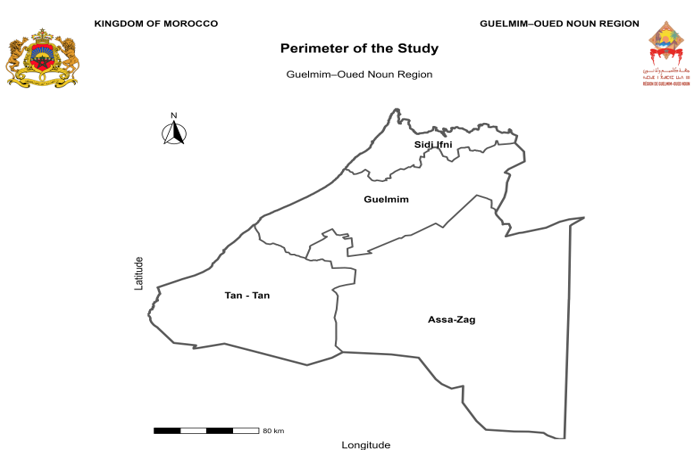
\includegraphics[width=0.85\textwidth]{image.png}
  \caption{Carte de la région Guelmim-Oued Noun}
  \label{fig:carte-region}
\end{figure}

\section{Le Recensement Général de la Population et de l'Habitat (RGPH)}

Le RGPH est la principale source de données démographiques et sociales au Maroc. Il permet de mesurer l'évolution de la population, de la structure des ménages, de la répartition urbaine et rurale, ainsi que les caractéristiques socio-économiques des ménages.

La version 2024 du RGPH fournit des informations détaillées pour chaque province et commune, et constitue la base de travail pour le tableau de bord développé pendant le stage.

\section{Enjeux territoriaux et indicateurs suivis}

Les indicateurs sélectionnés pour le tableau de bord sont les suivants :

\begin{itemize}[leftmargin=*]
  \item population totale et répartition par province ;
  \item population urbaine et rurale ;
  \item distribution par sexe ;
  \item structure par âge et pyramide des âges ;
  \item état matrimonial ;
  \item indicateurs de fécondité ;
  \item prévalence du handicap ;
  \item caractéristiques des ménages.
\end{itemize}

Ces indicateurs répondent aux besoins des décideurs pour l'évaluation des politiques publiques, la planification de l'offre de services et l'identification des zones les plus vulnérables.

\chapter{Analyse et Conception}

Cette section présente l'analyse des besoins, la conception fonctionnelle et la structure du tableau de bord.

\section{Analyse des besoins}

L'analyse des besoins a été réalisée à partir d'ateliers avec les agents du service statistique et des entretiens informels avec les responsables de suivi territorial. Les utilisateurs attendaient :

\begin{itemize}[leftmargin=*]
  \item une interface simple et accessible sans installation lourde ;
  \item des visualisations claires et comparables ;
  \item la possibilité d'accéder rapidement aux données par province et commune ;
  \item des indicateurs clés facilement exportables.
\end{itemize}

De plus, le besoin de synthèse était fort : la direction voulait un outil capable de mettre en évidence les tendances démographiques principales et les écarts territoriaux.

\section{Cahier des charges fonctionnel}

Le tableau de bord devait posséder les fonctionnalités suivantes :

\begin{enumerate}[leftmargin=*]
  \item navigation entre plusieurs thèmes : accueil, analyse régionale, population et sexe, structure par âge, état matrimonial, fécondité et handicap, ménages, et pages dédiées par province ;
  \item affichage de métriques synthétiques sous forme de cartes de valeur ;
  \item affichage de graphiques interactifs pour comparer les provinces et communes ;
  \item lecture directe des données depuis des fichiers Excel existants ;
  \item capacité à être déployé en interne sur un poste ou un serveur léger.
\end{enumerate}

Le design devait respecter une charte sobre et professionnelle, en cohérence avec l'identité du HCP et des documents officiels régionaux.

\section{Architecture logicielle}

Pour répondre aux attentes, le choix technique s'est porté sur une architecture légère basée sur Python :

\begin{itemize}[leftmargin=*]
  \item Streamlit pour l'interface web et la navigation ;
  \item pandas pour le chargement et le traitement des données Excel ;
  \item Plotly pour les graphiques interactifs ;
  \item fichiers Excel existants comme source de vérité des données.
\end{itemize}

Ce choix présente plusieurs avantages : déploiement rapide, faible maintenance, compatibilité avec les compétences déjà présentes dans l'équipe et possibilité d'évolution.

\section{Structuration des données}

Le dataset principal est un fichier Excel multi-onglets `RGPH__2024.xlsx`. Les onglets utilisés sont les suivants :

\begin{itemize}[leftmargin=*]
  \item `Population`
  \item `population urbaine_rurale`
  \item `menage par province`
  \item `masculin_féminin`
  \item `pyramide_ages_region`
  \item `age`
  \item `État Matrimonial`
  \item `mariage`
  \item `fecondite`
  \item `handicap_sexe`
  \item `handicap_province`
  \item `Ménages_Urbains`
  \item `guelmim_population`, `guelmim_sexe`, `guelmim_fecondite`, `guelmim_handicap`
  \item `sidi ifni_population`, `sidi ifni_sexe`, `sidi ifni_fecondite`, `sidi ifni_handicap`
  \item `tantan_population`, `tantan_sexe`, `tantan_fecondite`, `tantan_handicap`
  \item `assa zag_population`, `assa zag_sexe`, `assa sag_fecondite`, `assa zag_handicap`
\end{itemize}

La nomenclature, la cohérence des noms de colonnes et l'intégrité des formats numériques ont été vérifiées afin d'éviter des erreurs de lecture.

\section{Conception de l'interface utilisateur}

L'interface est organisée selon un modèle de navigation par onglets. Chaque page du tableau de bord présente un thème précis et une combinaison d'indicateurs.

La page d'accueil fait office de tableau de bord synthétique en présentant :

\begin{itemize}[leftmargin=*]
  \item un en-tête institutionnel ;
  \item une carte régionale ;
  \item un tableau de l'organisation administrative ;
  \item des cartes de présentation des provinces ;
  \item une brève présentation de l'objectif du projet.
\end{itemize}

Les pages thématiques suivantes combinent métriques numériques et visualisations graphiques.

\chapter{Réalisation}

Ce chapitre détaille les outils techniques, le développement et les choix mis en oeuvre pendant le stage.

\section{Environnement technique}

L'environnement de développement est composé de :

\begin{itemize}[leftmargin=*]
  \item Python 3.11+ ;
  \item Streamlit 1.30+ ;
  \item pandas 2.x ;
  \item Plotly 6.x ;
  \item un éditeur de code comme VS Code ;
  \item données sources au format Excel.
\end{itemize}

\section{Organisation du code}

L'application est contenue dans un script principal `app.py`. Ce script est structuré comme suit :

\begin{itemize}[leftmargin=*]
  \item importation des bibliothèques ;
  \item configuration de la page avec `st.set_page_config` ;
  \item définition de la source de données Excel ;
  \item fonction de chargement des données cachée avec `@st.cache_data` ;
  \item création de l'interface utilisateur via `st.sidebar.selectbox` ;
  \item navigation conditionnelle selon la sélection de l'utilisateur ;
  \item chargement des différents onglets Excel sur chaque page ;
  \item génération des figures Plotly et affichage avec `st.plotly_chart`.
\end{itemize}

\section{Traitement des données dans pandas}

Le traitement des données repose sur pandas pour assurer :

\begin{itemize}[leftmargin=*]
  \item la lecture des onglets Excel à l'aide de `pd.read_excel` ;
  \item la conversion des colonnes en types numériques appropriés ;
  \item le calcul de totaux et de ratios lorsque nécessaire ;
  \item le tri des données pour améliorer la lisibilité des graphiques ;
  \item l'ajout de colonnes calculées, comme le total des ménages par province.
\end{itemize}

Dans certains cas, des données ont été corrigées manuellement après vérification de la structure des feuilles Excel.

\section{Visualisation avec Plotly}

Plotly a été utilisé pour produire des graphiques interactifs. Les principaux types de visualisations sont :

\begin{itemize}[leftmargin=*]
  \item barres simples et groupées ;
  \item diagrammes en secteurs (pie et donut) ;
  \item pyramide des âges horizontale ;
  \item métriques numériques avec `st.metric`.
\end{itemize}

La palette de couleurs et les arrière-plans ont été harmonisés avec le thème sombre `plotly_dark` pour donner une apparence professionnelle.

\section{Pages thématiques}

Chaque page du tableau de bord présente des indicateurs spécifiques :

\subsection{Analyse Régionale}

Cette page agrège les données de population, d'urbanisation et de ménages au niveau régional et province. Elle permet de comparer la contribution de chaque province à la population totale.

\subsection{Population et Sexe}

La page de la répartition par sexe met en évidence l'équilibre hommes/femmes au niveau provincial et régional. Elle incorpore des graphiques groupés et un diagramme en anneau pour une lecture immédiate.

\subsection{Structure par Âge}

La pyramide des âges régionale et la répartition par grands groupes d'âge aident à comprendre la jeunesse de la population et le profil démographique. Cette page est essentielle pour les projections de demande scolaire et de services de santé.

\subsection{État Matrimonial}

L'analyse de l'état matrimonial permet d'identifier les catégories dominantes : célibataires, mariés, divorcés, veufs/veuves. Ces données sont utiles pour le suivi des politiques familiales et des actions sociales.

\subsection{Fécondité et Handicap}

Cette page suit l'indicateur conjoncturel de fécondité, la descendance finale des femmes et la prévalence du handicap. Elle compare également les taux de handicap entre les sexes et par province.

\subsection{Ménages}

L'analyse des ménages distingue les ménages urbains et ruraux, et calcule les totaux régionaux. Elle met en relief les déséquilibres territoriaux en termes de logement et d'accès aux services.

\subsection{Pages provinciales}

Quatre pages dédiées présentent des indicateurs détaillés pour chaque province :

\begin{itemize}[leftmargin=*]
  \item Province de Guelmim ;
  \item Province de Sidi Ifni ;
  \item Province de Tan-Tan ;
  \item Province d'Assa-Zag.
\end{itemize}

Sur chaque page, la population totale, urbaine, rurale, le nombre de ménages, la répartition par sexe, la fécondité et la prévalence du handicap sont affichés. Ces pages permettent un diagnostic territorial précis.

\section{Qualité et robustesse du code}

Le code a été conçu pour être facilement maintenable. Les éléments suivants ont été pris en considération :

\begin{itemize}[leftmargin=*]
  \item utilisation d'une fonction de chargement de données mise en cache ;
  \item standardisation des graphismes et des styles ;
  \item commentaires dans le script pour faciliter la lecture ;
  \item découpage logique en sections de page pour faciliter les évolutions.
\end{itemize}

Des tests manuels ont été réalisés après chaque modification pour s'assurer de l'absence de régression et de l'intégrité des visualisations.

\chapter{Analyse des résultats}

Cette partie commente les principaux résultats fournis par le tableau de bord et propose une interprétation des indicateurs.

\section{Population totale et répartition provinciale}

La région Guelmim-Oued Noun compte environ 448 685 habitants selon les données utilisées. La province de Guelmim représente la part la plus importante de la population régionale grâce à son chef-lieu et son bassin économique.

La comparaison entre provinces montre des écarts significatifs en termes de densité et de concentration urbaine. Les provinces littorales présentent des taux d'urbanisation plus élevés que les provinces sahariennes.

\section{Urbanisation et milieu de vie}

Le tableau de bord met en évidence une population urbaine majoritaire, avec environ 299 543 habitants en milieu urbain et 149 142 habitants en milieu rural. Cela confirme l'importance des pôles urbains comme moteurs de développement régional.

La distinction entre ménages urbains et ruraux est également primordiale pour planifier les infrastructures, la couverture en eau, l'électricité et les services de santé.

\section{Répartition par sexe}

La région présente une légère majorité féminine, avec 50,7\% de femmes contre 49,3\% d'hommes. Ce déséquilibre est faible, mais il est utile à suivre pour les politiques de genre et d'emploi.

La visualisation par province montre que les écarts sexe sont relativement stables, ce qui traduit une répartition homogène entre les territoires.

\section{Structure par âge}

La pyramide des âges révèle la présence d'une base jeune, typique des populations en transition démographique. Les groupes d'âge inférieurs à 20 ans représentent une part importante de la population.

Cette structure impose des besoins accrus en matière d'éducation, de formation professionnelle et d'emploi des jeunes dans les années à venir.

\section{État matrimonial}

Les données indiquent que 56,8\% de la population régionale est mariée, 34,4\% est célibataire, 3,3\% est divorcée et 5,5\% est veuve ou veuf. Ces statistiques sont essentielles pour comprendre les dynamiques familiales et la structure des ménages.

Le taux de mariage et la moyenne d'âge au premier mariage (30,60 ans) sont des indicateurs utiles pour les politiques de soutien à la famille et aux jeunes couples.

\section{Fécondité et handicap}

L'indicateur conjoncturel de fécondité est de 1,89, ce qui se situe dans la fourchette basse des nations en développement et suggère une dynamique démographique moins intense que par le passé.

La prévalence du handicap est estimée à 4,60\% au niveau régional, avec des taux proches entre les hommes et les femmes. La cartographie par province permet d'identifier les territoires où l'accompagnement des personnes en situation de handicap doit être renforcé.

\section{Analyse des ménages}

Le total des ménages régionaux est évalué à 105 394, avec une part importante de ménages urbains. La comparaison des ménages urbains et ruraux par province fait ressortir des disparités structurelles : certaines provinces concentrent des ménages urbains plus nombreux, tandis que d'autres sont marquées par une forte ruralité.

Ces éléments sont précieux pour la planification des politiques de logement social et des infrastructures de proximité.

\chapter{Étude de cas provinciale}

Ce chapitre met en exergue les principales caractéristiques démographiques des provinces de la région.

\section{Province de Guelmim}

La province de Guelmim est la plus peuplée de la région, avec une population totale de 196 267 habitants. Elle présente une urbanisation marquée, avec 153 238 habitants en zone urbaine et 43 029 en zone rurale.

La province est également caractérisée par des indicateurs de fécondité et de handicap qui nécessitent une attention particulière dans les politiques sociales.

\section{Province de Sidi Ifni}

La province de Sidi Ifni compte 104 601 habitants, avec une majorité rurale. La population urbaine est moindre, ce qui permet d'identifier des besoins spécifiques en matière de services de base et de développement local.

La présentation par commune sur cette page aide à localiser les zones de concentration démographique et à orienter les interventions.

\section{Province de Tan-Tan}

Avec 100 134 habitants, Tan-Tan se distingue par une urbanisation plus affirmée (85 410 habitants en zone urbaine). Ce profil impose des priorités en matière de transport, d'habitat et d'équipements urbains.

L'analyse de la fécondité locale et de la prévalence du handicap contribue à mieux adapter les programmes sociaux.

\section{Province d'Assa-Zag}

La province d'Assa-Zag est moins peuplée, avec 53 298 habitants, mais présente une forte ruralité et un contexte saharien. Le développement de cette province requiert une approche territoriale adaptée aux contraintes climatiques et aux mobilités longues.

Les indicateurs par commune révèlent les territoires les plus fragiles et les axes prioritaires pour l'aménagement du territoire.

\chapter{Discussion et enseignements}

Cette section propose une réflexion sur les apports du tableau de bord et sur les limites du projet.

\section{Apports du tableau de bord}

L'application développée apporte plusieurs contributions :

\begin{itemize}[leftmargin=*]
  \item démocratisation de l'accès aux indicateurs RGPH 2024 ;
  \item visualisation synthétique des dynamiques démographiques régionales ;
  \item support d'aide à la décision pour les services techniques ;
  \item base de travail pour des analyses futures sur les périmètres provinciaux.
\end{itemize}

Le format interactif favorise la compréhension des résultats par les utilisateurs non spécialistes des statistiques.

\section{Limites et contraintes}

Le projet présente plusieurs limites :

\begin{itemize}[leftmargin=*]
  \item dépendance aux fichiers Excel existants, dont la qualité peut varier ;
  \item absence de mise à jour automatique des données en temps réel ;
  \item certaines métriques sont encore partiellement codées en dur plutôt que calculées dynamiquement ;
  \item couverture limitée aux indicateurs disponibles dans le RGPH 2024.
\end{itemize}

Pour une version future, il conviendrait de renforcer la robustesse du traitement des données et de prévoir une intégration en base de données.

\section{Enseignements personnels}

Ce stage a permis de consolider plusieurs compétences :

\begin{itemize}[leftmargin=*]
  \item maîtrise de l'écosystème Python pour la data visualisation ;
  \item compréhension des enjeux démographiques territoriaux ;
  \item rigueur dans la préparation des données et la validation des résultats ;
  \item communication des résultats à des interlocuteurs non techniques.
\end{itemize}

L'expérience a également renforcé l'importance de la collaboration entre les acteurs statistiques et les décideurs locaux.

\chapter{Recommandations et perspectives}

Cette dernière partie propose des pistes d'amélioration et des prolongements pour le projet.

\section{Améliorations techniques}

Les évolutions possibles du tableau de bord incluent :

\begin{itemize}[leftmargin=*]
  \item refactoring du code pour extraire les fonctions récurrentes ;
  \item ajout d'un module de nettoyage et de validation automatique des données ;
  \item ajout d'une couche d'exportation des tableaux et graphiques au format PDF ou Excel ;
  \item migration vers une base de données relationnelle pour gérer les mises à jour successives du RGPH.
\end{itemize}

\section{Extensions fonctionnelles}

Des fonctionnalités supplémentaires pourraient être ajoutées :

\begin{itemize}[leftmargin=*]
  \item carte interactive par commune ;
  \item comparaison temporelle avec les recensements précédents ;
  \item indicateurs socio-économiques complémentaires (emploi, éducation, santé) ;
  \item module d'analyse prédictive des effectifs scolaires et des besoins en logement.
\end{itemize}

\section{Pistes de recherche}

Le rapport ouvre des pistes de recherche plus longues :

\begin{itemize}[leftmargin=*]
  \item analyse des trajectoires démographiques des communes sahariennes ;
  \item évaluation de l'impact des politiques de régionalisation sur les migrations internes ;
  \item modélisation des besoins en infrastructure selon les scénarios de croissance démographique.
\end{itemize}

\chapter{Conclusion Générale}
\addcontentsline{toc}{chapter}{Conclusion Générale}

Le projet de tableau de bord démographique réalisé au sein de la Direction Régionale du HCP de Guelmim constitue une contribution utile pour la visualisation et l'analyse des données territoriales du RGPH 2024. L'outil offre un cadre simple et efficace pour suivre les indicateurs principaux, comparer les provinces et soutenir la réflexion stratégique.

La réalisation a permis de mettre en pratique des compétences en développement Python, traitement de données et visualisation. Les résultats confirment l'intérêt d'une solution interactive pour rapprocher les statistiques des décideurs et des projets d'aménagement.

Le travail peut être prolongé par une automatisation des flux de données, l'ajout de nouvelles dimensions analytiques et le déploiement d'une version pérenne accessible aux équipes régionales.

% ==========================================
% BIBLIOGRAPHIE
% ==========================================
\clearpage
\printbibliography[heading=bibintoc,title={Bibliographie}]

% ==========================================
% ANNEXES
% ==========================================
\clearpage
\appendix

\chapter{Annexe A : Captures d’écran}
Cette annexe présente des captures d'écran illustrant l'interface et les résultats du tableau de bord.

\begin{figure}[H]
  \centering
  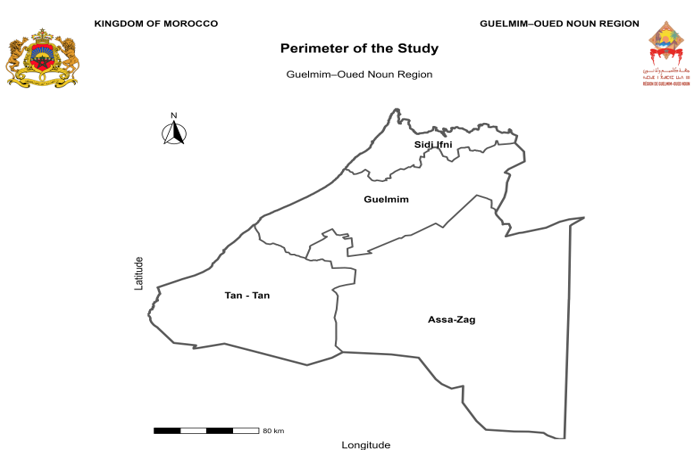
\includegraphics[width=0.85\textwidth]{image.png}
  \caption{Exemple de visuel d'accueil du dashboard}
  \label{fig:capture-accueil}
\end{figure}

\section{Capture d’écran 1}
La capture d'écran illustre la page d'accueil avec la structure administrative et les provinces de la région.

\section{Capture d’écran 2}
La capture d'écran présente une page d'analyse régionale avec des graphiques de population.

\chapter{Annexe B : Extraits de code source}
Ajout d'extraits importants du code source pour documenter la logique de chargement de données et de génération des graphiques.

\section{Chargement des données}
\begin{verbatim}
@st.cache_data
def load_home_data():
    return pd.read_excel(excel_file, sheet_name="Population")

pop = load_home_data()
\end{verbatim}

\section{Page d'analyse régionale}
\begin{verbatim}
if page == "Analyse Régionale":
    st.title("Tableau de Bord Démographique de la Région Guelmim-Oued Noun")
    st.write("---")
    col1, col2, col3, col4 = st.columns(4)
    with col1:
        st.metric(label="Population totale", value="448 685")
    ...
\end{verbatim}

\chapter{Annexe C : Tables et nomenclature}

\begin{table}[H]
  \centering
  \caption{Répartition des provinces et communes de la région}
  \begin{tabular}{lcc}
    \toprule
    Province & Cercles & Communes \\
    \midrule
    Guelmim & 3 & 20 \\
    Sidi Ifni & 2 & 19 \\
    Tan-Tan & 2 & 7 \\
    Assa-Zag & 2 & 7 \\
    \bottomrule
  \end{tabular}
  \label{tab:provinces}
\end{table}

\section{Nomenclature des abréviations}
Ce rapport utilise les abréviations suivantes :

\begin{itemize}[leftmargin=*]
  \item API : Application Programming Interface ;
  \item CNN : Convolutional Neural Network ;
  \item IDS : Intrusion Detection System ;
  \item SQL : Structured Query Language ;
  \item HCP : Haut-Commissariat au Plan ;
  \item DUT : Diplôme Universitaire de Technologie ;
  \item ML : Machine Learning ;
  \item IA : Intelligence Artificielle ;
  \item RGPH : Recensement Général de la Population et de l'Habitat.
\end{itemize}

\chapter{Annexe D : Documents complémentaires}

Les documents complémentaires incluent les rapports internes du HCP, les extraits du RGPH 2024, ainsi que les notes méthodologiques utilisées pendant le stage.

\end{document}
